\documentclass[a4paper]{scrreprt}
%\documentclass[a4paper]{report}

% Uncomment to optimize for double-sided printing.
% \KOMAoptions{twoside}

% Set binding correction manually, if known.
% \KOMAoptions{BCOR=2cm}

% Localization options
\usepackage[english]{babel}
\usepackage[T1]{fontenc}
\usepackage[utf8]{inputenc}

% Enhanced verbatim sections. We're mainly interested in
% \verbatiminput though.
\usepackage{verbatim}

% PDF-compatible landscape mode.
% Makes PDF viewers show the page rotated by 90°.
\usepackage{pdflscape}

% Advanced tables
\usepackage{tabu}
\usepackage{longtable}

% Fancy tablerules
\usepackage{booktabs}

% Graphics
\usepackage{graphicx}

% Current time
\usepackage[useregional=numeric]{datetime2}

% Float barriers.
% Automatically add a FloatBarrier to each \section
\usepackage[section]{placeins}

% Custom header and footer
\usepackage{fancyhdr}
\setlength{\headheight}{15.2pt}
\pagestyle{fancyplain}

\usepackage{geometry}
\usepackage{layout}

% Math tools
\usepackage{mathtools}
% Math symbols
\usepackage{amsmath,amsfonts,amssymb}

\fancyhf{}
% Chapter header on non-plain pages only.
\lhead{\fancyplain{} {\leftmark}}
% Footer must contain print date. Ugly, but IPA requirement.
\lfoot{\printdate}
% Print date left and page count right was the thing which looked the
% most balanced.
\rfoot{\thepage}
% 
% Source code & highlighting
\usepackage{listings}

% Convenience commands
\newcommand{\mailsubject}{2407 - Computernetze - Practical exercise 2}
\newcommand{\maillink}[1]{\href{mailto:#1?subject=\mailsubject}
                               {#1}}

% Should use this command wherever the print date is mentioned.
\newcommand{\printdate}{\today}

\subject{2407 - Computernetze}
\title{Practical exercise 2}

\author{Michael Senn \maillink{michael.senn@students.unibe.ch}}

\date{\printdate}

% Needs to be the last command in the preamble, for one reason or
% another. 
\usepackage{hyperref}


\begin{document}
\maketitle

% \tableofcontents

\chapter{Throughput measurements}

Using iPerf - a free and open-source tool allowing to measure bandwith of IP
networks - simultaneous IPv4 throughput between VM1 and VM2, as well as VM3 and
VM2, was measured.

\section{iPerf server}

On VM2 an iPerf server was started via \texttt{iperf -s}. By default the iPerf
server will listen for incoming TCP connections on port 5001.

\section{iPerf clients}

On VM1 and VM3 respectively, iPerf clients were started via \texttt{iperf -c
10.0.2.2} - \texttt{10.0.2.2} being the IP of VM2, where the iPerf server was
running.

In order to ensure that the two throughput tests happened as simultaneously as
possible, \texttt{sleep} was used on one of the VMs, which made the VM wait a
configurable amount of seconds before executing the following command. This
allowed for plenty of time to switch to the second VM and, as soon as the iPerf
client started on the first VM, quickly start it on the second VM too.

A total of four measurements were made, with two per VM having had the iPerf
client launched manually, and the other two having had the iPerf client
launched via \texttt{sleep}. This should serve to even out the impact of the
slight delay due to manually triggering the measurement on one machine.

If one wanted to increase accuracy even further, it would be possible to
synchronize the two VM's clocks to the same source, and trigger the iPerf
measurement programatically based on the respective machine's time.

\section{Results}

\begin{figure}
    \centering
    \textbf{iPerf server on VM2}\par\medskip
    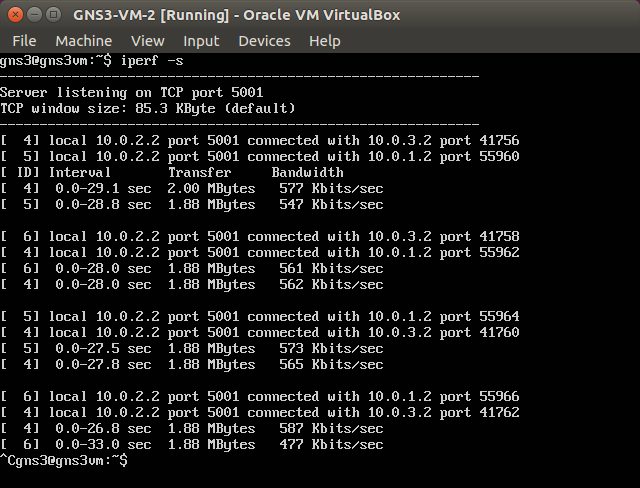
\includegraphics[width=\textwidth]{resources/iperf_server_vm2.png}
\end{figure}

\begin{figure}
    \centering
    \textbf{iPerf client on VM1}\par\medskip
    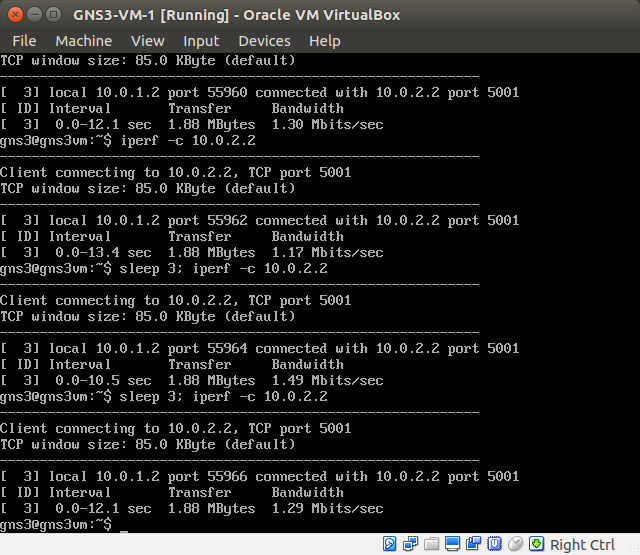
\includegraphics[width=\textwidth]{resources/iperf_vm1.png}
\end{figure}

\begin{figure}
    \centering
    \textbf{iPerf client on VM3}\par\medskip
    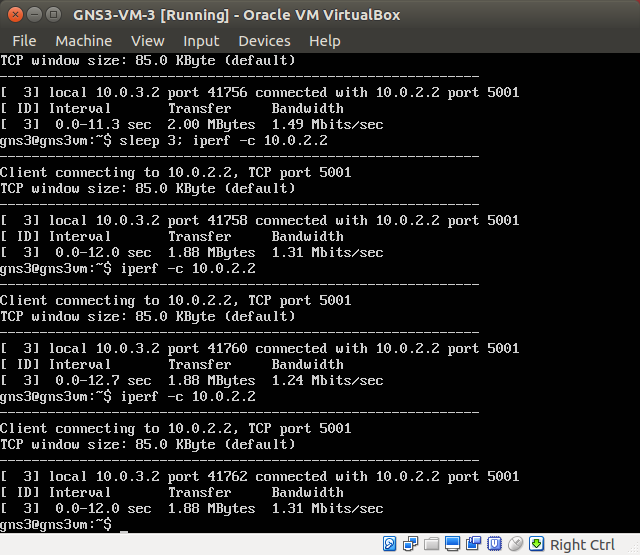
\includegraphics[width=\textwidth]{resources/iperf_vm3.png}
\end{figure}

\begin{figure}
    \centering
    \textbf{Wireshark conversation view on Hub 2}\par\medskip
    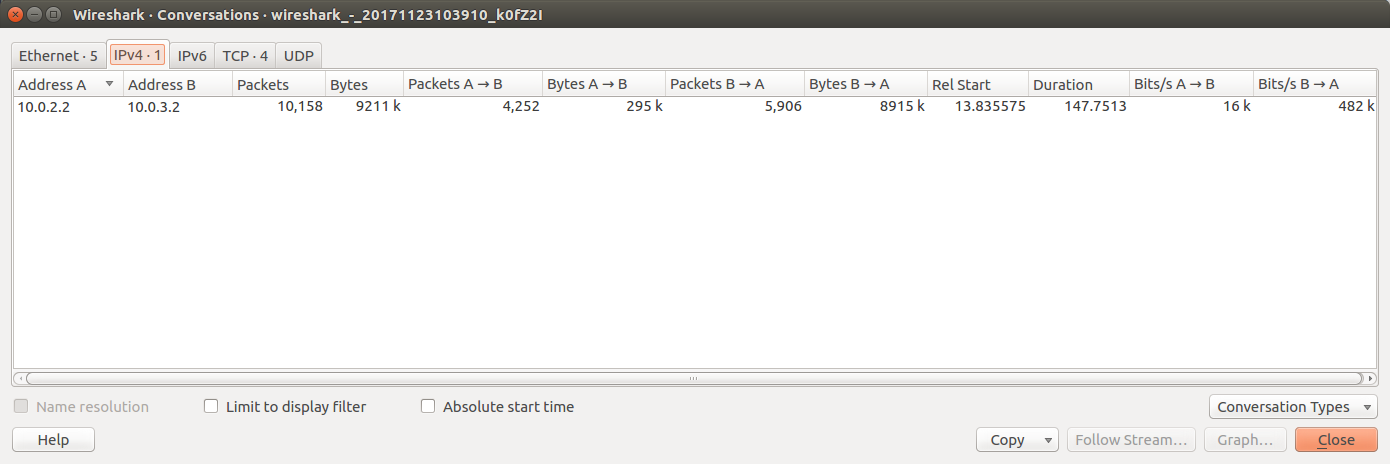
\includegraphics[width=\textwidth]{resources/hub_2_conversation.png}
\end{figure}

The maximum observed total throughput was 2.79 Mbit/s which, with the routers
supporting FastEthernet, which has a maximum theoretical throughput of 100
Mbit/s, is surprisingly low. Even with protocol overhead it seems as if there
is either a component involved which does not support FastEthernet, or that the
duplicate virtualization simply leads to lackluster performance.

\subsection{Jain's fairness index}

Calculating Jain's fairness index, which is defined as

\begin{displaymath}
	\tau(x_1, x_2, \dots, x_n) = \frac{(\sum_{i = 1}^{n} x_i)^2}{n \cdot \sum_{i = 1}^{n} x_i^2}
\end{displaymath}

,using the values gathered during the four measurements, leads to the following
results when rounded to three digits:
\\
\\
\begin{tabular}{|c|c|c|c|}
	\hline
	Measurement & Throughput VM1 & Throughput VM3 & Jain's Fairness Index \\
	\hline
	1 & 1.30 Mbit/s & 1.49 Mbit/s & 0.995 \\
	2 & 1.17 Mbit/s & 1.31 Mbit/s & 0.997 \\
	3 & 1.49 Mbit/s & 1.24 Mbit/s & 0.992 \\
	4 & 1.29 Mbit/s & 1.31 Mbit/s & 1.0 \\
	\hline
\end{tabular}

Using the average throughput values, which are 1.3125 Mbit/s for VM1, and
1.3375 Mbit/s for VM3, leads to a fairness index of 1.0.

\end{document}
